% Compile with XeLaTeX or LuaLaTeX (fontspec is used for IPA/Greek glyphs).
%   latexmk -xelatex slides.tex
% Reuses ../figures/*.pdf and ../tables/*.tex from the paper build.
\documentclass[aspectratio=169]{beamer}

\usetheme{Madrid}
\usecolortheme{seahorse}
\setbeamertemplate{navigation symbols}{}
\setbeamertemplate{caption}{\raggedright\insertcaption\par}

\usepackage{graphicx}
\usepackage{booktabs}
\usepackage{amsmath,amssymb}
\usepackage{fontspec}
\IfFileExists{fonts/DejaVuSans.ttf}
  {\newfontfamily\ipafont[Path=fonts/]{DejaVuSans.ttf}}
  {\IfFontExistsTF{DejaVu Sans}{\newfontfamily\ipafont{DejaVu Sans}}{\let\ipafont\relax}}
\newcommand{\ipa}[1]{{\ipafont #1}}

\title[LoRA for Multilingual G2P]{LoRA for Multilingual Grapheme-to-Phoneme Conversion}
\subtitle{Parameter-Efficient Adaptation of ByT5-G2P on Romanian and Modern Greek}
\author[Tudor, Stoian]{Dan-Gabriel Tudor \and \c{S}tefan-Rare\c{s} Stoian}
\institute[UB]{Faculty of Mathematics and Informatics \\ University of Bucharest}
\date{2026}

\begin{document}

\begin{frame}[plain]
  \titlepage
  \begin{center}\scriptsize
  \url{https://github.com/stoianraresstefan/G2P-Parameter-Efficient-Fine-Tuning}
  \end{center}
\end{frame}

\begin{frame}{The grapheme-to-phoneme (G2P) task}
  \begin{itemize}
    \item G2P maps spelling to pronunciation, a phoneme sequence (IPA).
    \item It is the front-end of \alert{text-to-speech} and supplies the lexicons behind \alert{speech recognition}.
    \item Example: Romanian \emph{porne\c{s}te} ``[it] starts'' $\rightarrow$ \ipa{p o r n e ʃ t e}, where \emph{\c{s}} $\rightarrow$ \ipa{/ʃ/}.
    \item Spelling-to-sound mappings are irregular even in ``shallow'' orthographies, so G2P is nontrivial.
  \end{itemize}
\end{frame}

\begin{frame}{Why multilingual G2P matters}
  \begin{itemize}
    \item High-quality pronunciation lexicons need linguistic expertise and are \alert{scarce} for most languages.
    \item Pretrained multilingual models (CharsiuG2P / ByT5-G2P) transfer orthographic and phonological regularities across $\sim$100 languages from \alert{one} network.
    \item They are strong off the shelf --- but still benefit from \alert{per-language adaptation} when in-language data exists.
  \end{itemize}
\end{frame}

\begin{frame}{The cost problem}
  \begin{itemize}
    \item Adapting by \alert{full fine-tuning} stores a complete copy of $\sim$300M weights \emph{per language}: $K$ languages $\Rightarrow K\times 300$M.
    \item It can also \alert{overwrite} previously learned languages (catastrophic forgetting).
    \item Parameter-efficient fine-tuning (PEFT) --- LoRA, adapters --- is standard for LLMs and ASR\ldots
    \item \ldots but has \alert{not} been adopted for G2P. \textbf{That is the gap we study.}
  \end{itemize}
\end{frame}

\begin{frame}{Research question}
  \begin{block}{}
    \centering\large
    Can \alert{LoRA} match \alert{full fine-tuning} of ByT5-G2P on low-resource languages while training \alert{under 1\%} of the parameters --- and how do they compare on \alert{catastrophic forgetting}?
  \end{block}
  \vspace{1em}
  \begin{itemize}
    \item First systematic study of LoRA for multilingual G2P.
    \item Measured on Romanian and Modern Greek (SIGMORPHON 2021, low-resource).
  \end{itemize}
\end{frame}

\begin{frame}{Method: one model, four adaptation strategies}
  Base model: \textbf{CharsiuG2P ByT5-small} ($\sim$300M params, byte-level, no language-specific vocabulary).
  \vspace{0.5em}
  \begin{itemize}
    \item \textbf{Zero-shot} --- pretrained model, no training (0\%).
    \item \textbf{Frozen head} --- train only the LM head (0.19\%).
    \item \textbf{LoRA} --- low-rank updates on attention q/k/v/o, $r\in\{8,16\}$, $\alpha{=}2r$ (0.39--0.78\%): $W + \tfrac{\alpha}{r}BA$.
    \item \textbf{Full fine-tuning} --- all parameters (100\%).
  \end{itemize}
  \vspace{0.3em}
  Greedy decoding; input prompt \texttt{<ron>:}\,/\,\texttt{<gre>:}.
\end{frame}

\begin{frame}{Data and experimental setup}
  \begin{itemize}
    \item \textbf{SIGMORPHON 2021}, low-resource: Romanian (Latin / Romance) and Greek (Greek script / Hellenic) --- 800/100/100 words, IPA targets.
    \item \textbf{Metrics:} PER (character-level edit rate) and WER; \alert{forgetting} measured on held-out English (\texttt{eng-us}) IPA.
    \item \textbf{Compute:} Kaggle dual T4 GPUs; HuggingFace \texttt{transformers} + \texttt{peft}.
    \item Two fixes that mattered: the ISO-639-3 tag \texttt{<ron>} (not the file code \texttt{rum}; $5.96$ vs $24.76$ dev PER), and character-level scoring so the un-delimited zero-shot output is comparable.
  \end{itemize}
\end{frame}

\begin{frame}{Main results}
  \begin{center}
  \resizebox{\textwidth}{!}{\begin{tabular}{lcccc}
\toprule
 & \multicolumn{2}{c}{Romanian} & \multicolumn{2}{c}{Greek} \\
\cmidrule(lr){2-3}\cmidrule(lr){4-5}
Method & PER & WER & PER & WER \\
\midrule
Zero-shot & 4.48 & 22.00 & \textbf{1.56} & \textbf{10.00} \\
Frozen head & 4.48 & 23.00 & 1.71 & 11.00 \\
LoRA (r=8) & 4.11 $\pm$ 0.20 & 18.67 $\pm$ 2.36 & 7.32 & 35.00 \\
LoRA (r=16) & 3.36 & 15.00 & 7.17 & 35.00 \\
Full FT & \textbf{1.76} & \textbf{10.00} & 2.80 & 16.00 \\
\midrule
Baseline & -- & 10.00 & -- & 21.00 \\
\bottomrule
\end{tabular}
}
  \end{center}
  \vspace{0.3em}
  \footnotesize
  \begin{itemize}
    \item \textbf{Romanian:} adaptation helps --- full FT best (PER 1.76, WER 10), LoRA $r{=}16$ (3.36) beats zero-shot (4.48) at \alert{0.78\%} of params.
    \item \textbf{Greek:} zero-shot already excellent (PER 1.56); no fine-tuning improves it.
  \end{itemize}
\end{frame}

\begin{frame}{Accuracy vs.\ cost: the Pareto view}
  \begin{center}
  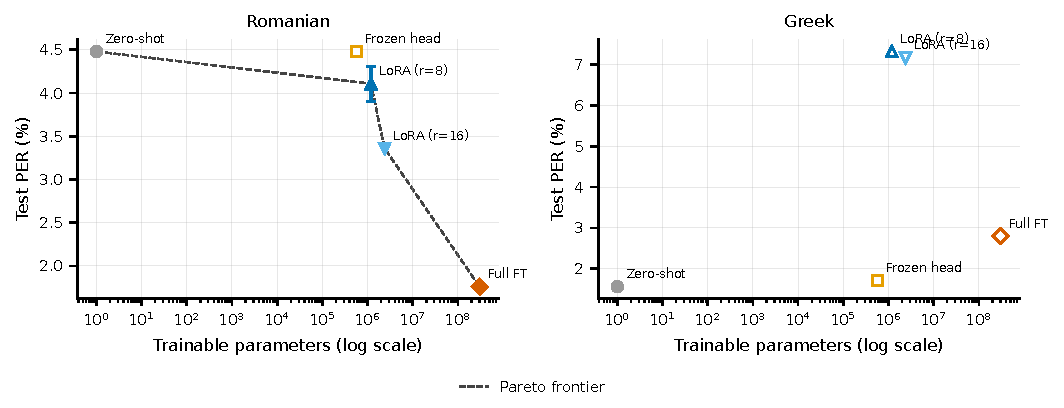
\includegraphics[width=0.92\linewidth]{../figures/fig1_pareto}
  \end{center}
  \vspace{-0.3em}
  \footnotesize Romanian: each extra parameter budget buys lower PER. \quad Greek: zero-shot dominates the frontier.
\end{frame}

\begin{frame}{Catastrophic forgetting on English}
  \begin{columns}
    \begin{column}{0.55\textwidth}
      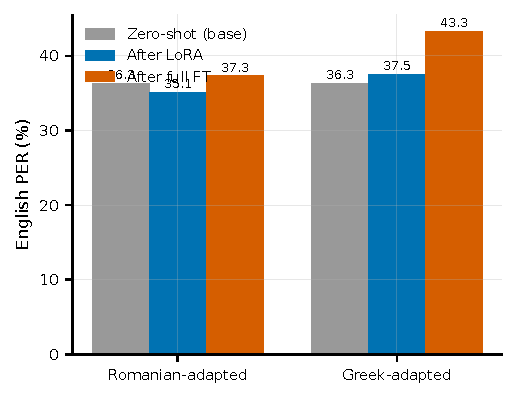
\includegraphics[width=\linewidth]{../figures/fig2_forgetting}
    \end{column}
    \begin{column}{0.45\textwidth}
      \begin{itemize}
        \item Base model: PER \textbf{36.3}.
        \item \alert{Full fine-tuning forgets most} (Greek-adapted 43.3, $+7$).
        \item \textbf{LoRA / frozen-head stay near baseline.}
        \item Frozen base $\Rightarrow$ multilingual ability preserved.
      \end{itemize}
      \centering\small The cleanest argument for PEFT.
    \end{column}
  \end{columns}
\end{frame}

\begin{frame}{Limitations and future work}
  \begin{itemize}
    \item \textbf{Scope:} two languages, two LoRA ranks, mostly single-seed, one base model, isolated words only, no adapter baseline.
    \item \textbf{Threat to validity:} Greek zero-shot is likely inflated by overlap between CharsiuG2P's WikiPron pretraining and the test set (within-split leakage is 0\% exact).
    \item \textbf{Metric:} character-level PER is internally consistent but not the official phoneme-token PER.
    \item \textbf{Future:} adapters and wider rank sweep; more languages/scripts; self-training; sentence-level G2P; robustness.
  \end{itemize}
\end{frame}

\begin{frame}{Conclusion}
  \begin{itemize}
    \item LoRA \alert{approaches full fine-tuning} where adaptation helps (Romanian PER $4.48\rightarrow3.36$) at \alert{$<1\%$} of the parameters.
    \item Per-language storage drops from $K\times{\sim}300$M to $K\times{\sim}1$--$2$M weights.
    \item By freezing the backbone, LoRA \alert{preserves the multilingual base} where full fine-tuning forgets it.
  \end{itemize}
  \vspace{0.6em}
  \begin{block}{Takeaway}
    \centering PEFT is a practical default for per-language G2P deployment.
  \end{block}
\end{frame}

\begin{frame}[plain]
  \centering
  \vfill
  {\Large Thank you --- Questions?}\\[1em]
  \footnotesize \url{https://github.com/stoianraresstefan/G2P-Parameter-Efficient-Fine-Tuning}
  \vfill
\end{frame}

\end{document}
